\documentclass[10pt,a4paper]{article}

\usepackage[T1]{fontenc}
\usepackage[utf8]{inputenc}
\usepackage{lmodern}
\usepackage{microtype}
\usepackage[a4paper,top=20mm,bottom=22mm,left=20mm,right=20mm,headheight=15pt]{geometry}
\usepackage{amsmath,amssymb,mathtools,amsthm}
\usepackage{booktabs,longtable,tabularx,array,multirow}
\usepackage{graphicx,float,caption,subcaption}
\usepackage{xcolor}
\usepackage{enumitem}
\usepackage{listings}
\usepackage{fancyhdr}
\usepackage{titlesec}
\usepackage{hyperref}
\usepackage[nameinlink,noabbrev]{cleveref}
\usepackage[most]{tcolorbox}
\usepackage{pdflscape}
\usepackage{ragged2e}
\usepackage{lastpage}

\definecolor{TKnavy}{HTML}{12313F}
\definecolor{TKteal}{HTML}{1F9E9E}
\definecolor{TKpurple}{HTML}{6E5A9B}
\definecolor{TKgold}{HTML}{D4A017}
\definecolor{TKcoral}{HTML}{CC6E5A}
\definecolor{TKgreen}{HTML}{4B8B68}
\definecolor{TKgray}{HTML}{5E6C73}
\definecolor{TKlight}{HTML}{F4F7F8}
\definecolor{TKwarning}{HTML}{FFF4D6}
\definecolor{TKreject}{HTML}{FBE9E5}

\hypersetup{
  colorlinks=true,
  linkcolor=TKpurple,
  urlcolor=TKteal,
  citecolor=TKcoral,
  pdftitle={Tom Klootwijk Chrono-Topological-Geometric Substrate and Manifold},
  pdfauthor={Requester attribution: Tom Klootwijk; formalization package v1.0.0},
  pdfsubject={Formal hybrid stratified substrate with KLB37, KLSC1 and KLOC1 implementation profiles},
  pdfkeywords={chrono-topological geometry, hybrid manifold, signed distance field, topology, event calculus, KLB37, KLSC1, KLOC1}
}

\pagestyle{fancy}
\fancyhf{}
\fancyhead[L]{\sffamily\bfseries\color{TKnavy}TK-CTG 1.0}
\fancyhead[R]{\sffamily\color{TKgray}Tom Klootwijk Manifold}
\fancyfoot[L]{\scriptsize\sffamily Requester-supplied attribution; not independently verified}
\fancyfoot[R]{\scriptsize\sffamily Page \thepage\ of \pageref*{LastPage}}
\renewcommand{\headrulewidth}{0.5pt}
\renewcommand{\footrulewidth}{0pt}

\titleformat{\section}{\Large\sffamily\bfseries\color{TKnavy}}{\thesection}{0.7em}{}
\titleformat{\subsection}{\large\sffamily\bfseries\color{TKteal}}{\thesubsection}{0.7em}{}
\titleformat{\subsubsection}{\normalsize\sffamily\bfseries\color{TKpurple}}{\thesubsubsection}{0.7em}{}
\titlespacing*{\section}{0pt}{2.4ex plus .5ex minus .2ex}{1.0ex}
\titlespacing*{\subsection}{0pt}{2.0ex plus .4ex minus .2ex}{0.7ex}

\setlist[itemize]{leftmargin=1.5em,itemsep=0.25em,topsep=0.35em}
\setlist[enumerate]{leftmargin=1.7em,itemsep=0.25em,topsep=0.35em}
\setlength{\parindent}{0pt}
\setlength{\parskip}{0.55em}
\renewcommand{\arraystretch}{1.18}

\newcolumntype{Y}{>{\RaggedRight\arraybackslash}X}
\newcolumntype{L}[1]{>{\RaggedRight\arraybackslash}p{#1}}
\newcolumntype{C}[1]{>{\Centering\arraybackslash}p{#1}}

\tcbset{fonttitle=\sffamily\bfseries,boxrule=0.8pt,arc=2mm,left=2mm,right=2mm,top=1.5mm,bottom=1.5mm}
\newtcolorbox{decisionbox}{enhanced,breakable,colback=TKlight,colframe=TKnavy,title=DECISION}
\newtcolorbox{boundarybox}{enhanced,breakable,colback=TKwarning,colframe=TKgold,title=BOUNDARY}
\newtcolorbox{correctionbox}{enhanced,breakable,colback=TKreject,colframe=TKcoral,title=CORRECTION}
\newtcolorbox{implementationbox}{enhanced,breakable,colback=white,colframe=TKteal,title=IMPLEMENTATION PROFILE}
\newtcolorbox{plainbox}[1]{enhanced,breakable,colback=white,colframe=TKgray,title=#1}

\newtcbtheorem[number within=section]{formaldef}{Formal Definition}{enhanced,breakable,colback=white,colframe=TKpurple,fonttitle=\sffamily\bfseries}{def}
\newtcbtheorem[number within=section]{proposition}{Proposition}{enhanced,breakable,colback=white,colframe=TKgreen,fonttitle=\sffamily\bfseries}{prop}
\newtcbtheorem[number within=section]{invariant}{Invariant}{enhanced,breakable,colback=TKlight,colframe=TKteal,fonttitle=\sffamily\bfseries}{inv}

\lstdefinestyle{tkcode}{
  basicstyle=\ttfamily\scriptsize,
  backgroundcolor=\color{TKlight},
  frame=single,
  rulecolor=\color{TKgray},
  breaklines=true,
  columns=fullflexible,
  keepspaces=true,
  showstringspaces=false,
  tabsize=2,
  keywordstyle=\color{TKpurple}\bfseries,
  commentstyle=\color{TKgreen},
  stringstyle=\color{TKcoral}
}
\lstdefinelanguage{json}{
  basicstyle=\ttfamily\scriptsize,
  string=[s]{"}{"},
  stringstyle=\color{TKcoral},
  comment=[l]{//},
  commentstyle=\color{TKgreen},
  morecomment=[s]{/*}{*/},
  literate=
   *{0}{{{\color{TKpurple}0}}}{1}
    {1}{{{\color{TKpurple}1}}}{1}
    {2}{{{\color{TKpurple}2}}}{1}
    {3}{{{\color{TKpurple}3}}}{1}
    {4}{{{\color{TKpurple}4}}}{1}
    {5}{{{\color{TKpurple}5}}}{1}
    {6}{{{\color{TKpurple}6}}}{1}
    {7}{{{\color{TKpurple}7}}}{1}
    {8}{{{\color{TKpurple}8}}}{1}
    {9}{{{\color{TKpurple}9}}}{1}
    {true}{{{\color{TKteal}\bfseries true}}}{4}
    {false}{{{\color{TKteal}\bfseries false}}}{5}
    {null}{{{\color{TKgray}\bfseries null}}}{4}
}
\lstset{style=tkcode}

\newcommand{\TKM}{\mathcal{M}_{\mathrm{TK}}}
\newcommand{\TKSub}{\mathfrak{S}_{\mathrm{TK}}}
\newcommand{\Time}{\mathbb{T}}
\newcommand{\Real}{\mathbb{R}}
\newcommand{\source}[1]{\textsf{\color{TKgray}[#1]}}
\newcommand{\code}[1]{\texttt{#1}}

\begin{document}

\hypersetup{pageanchor=false}
\begin{titlepage}
  \pagecolor{TKnavy}\color{white}
  \vspace*{14mm}
  {\sffamily\bfseries\fontsize{29}{34}\selectfont TOM KLOOTWIJK\par}
  \vspace{4mm}
  {\sffamily\bfseries\fontsize{25}{30}\selectfont CHRONO-TOPOLOGICAL-GEOMETRIC\par}
  {\sffamily\bfseries\fontsize{25}{30}\selectfont SUBSTRATE AND MANIFOLD\par}
  \vspace{8mm}
  {\sffamily\fontsize{15}{19}\selectfont Formal definition, evidence boundary, KLB implementation mapping and executable reference package\par}

  \vfill

  \begin{tcolorbox}[colback=white!8!TKnavy,colframe=TKteal,coltext=white,title=FORMAL CLASS]
  The \textbf{Tom Klootwijk Manifold} is defined here as a \textbf{hybrid stratified quotient state space}. Its regular pieces are time-extended geometric manifolds; explicit gluing maps and certified event transitions connect those pieces. It is globally smooth only when the declared regularity, Hausdorff and non-branching conditions hold.
  \end{tcolorbox}

  \vspace{4mm}
  \begin{tabularx}{\textwidth}{@{}L{42mm}Y@{}}
    \textbf{Version} & 1.0.0, 22 August 2026 \\
    \textbf{Requester attribution} & Tom Klootwijk; NL200678942; 10-07-1990; country marker NL \\
    \textbf{Attribution status} & Requester-supplied and not independently verified \\
    \textbf{Implementation basis} & KLB SeedChain GPU 0.3.0: KLB37, KLSC1 and KLOC1 \\
    \textbf{Core boundary} & No physical-causation, zero-cost, infinite-resolution, legal-authorship, identity-verification or navigation-grade claim \\
  \end{tabularx}

  \vfill
  {\sffamily\small Definitions, schemas, reference code, tests, diagrams, source hashes and checksums accompany this PDF.\par}
\end{titlepage}
\hypersetup{pageanchor=true}
\nopagecolor\color{black}

\pagenumbering{roman}
\setcounter{page}{1}

\section*{Abstract}
\addcontentsline{toc}{section}{Abstract}

This specification gives a precise meaning to the requester’s phrases \emph{chrono-topological-geometric substrate}, \emph{Tom Klootwijk Manifold}, \emph{SDF zero}, \emph{hinge}, \emph{parity/LSB route}, and \emph{chronotemporal latch}. It uses the literal referential architecture of UGTS-KC 3.6 as the governing evidence discipline, and it maps the resulting formal objects to the supplied KLB SeedChain GPU 0.3.0 implementation.

The substrate is a typed, content-addressed state-and-event system. Its geometric carrier is a disjoint union of mode-indexed manifolds; its topology is a set of explicit gluing and transport maps; its chronology is a declared time domain with deterministic flows or bounded predictors; and its dynamics are committed through support, compatibility, certified guard crossings, atomic transitions and ordered lineage. The named manifold is the quotient/geometric realization of that hybrid system. Because branches, merges, discrete sheets and event identifications may occur, the rigorous general category is a \emph{hybrid stratified topological state space}; the word \emph{manifold} names the defined construction but does not silently assert global smoothness.

The specification corrects several claims appearing in the dialogue sources. The equation \(f=0\) defines the zero-level set of the declared implicit field, not automatically a sphere. Generic implicit fields are not automatically exact signed-distance functions. Zero-based or LSB notation can select an address or route but does not reduce a numeric Hamming distance. A seven-dimensional Euclidean profile can carry seven mutually orthogonal axes, but the current KLB implementation reconstructs three-dimensional positions plus finite topology state. Compact procedural definitions can avoid materializing some dense state, but they still consume instructions, registers, cache and memory and do not prove constant-time rendering or zero VRAM.

\begin{decisionbox}
\textbf{Canonical notation.}
For a declared profile \(\Pi\), the Tom Klootwijk Manifold is
\[
\TKM(\Pi)
=\left(\bigsqcup_{q\in\mathcal Q}\Time\times M_q\times U_q\times\{q\}\right)\big/\!\sim_{\Gamma,\Delta},
\]
where \(\Gamma\) contains explicit boundary-port gluing maps and \(\Delta\) contains guarded event transitions. The surrounding substrate is
\[
\TKSub(\Pi)=
(\mathcal D,\mathcal A,\TKM(\Pi),\Phi,\mathcal F,\mathcal S,\mathcal C,\mathcal H,
\mathcal E,\Delta,\mathcal I,\mathcal L,\mathcal P,\mathcal B).
\]
All symbols are defined in \cref{sec:core,sec:manifold}.
\end{decisionbox}

\tableofcontents
\clearpage
\pagenumbering{arabic}

\section{Scope, source basis and evidence discipline}
\label{sec:scope}

\subsection{Requested object}

The requested deliverable is not a claim that a new physical law has been experimentally established. It is a formal definition and implementation mapping for a named mathematical/computational object discussed across the supplied documents. The package therefore distinguishes four layers:

\begin{enumerate}
  \item \textbf{source-derived structure}: objects stated cleanly in UGTS-KC 3.6 or implemented in KLB 0.3.0;
  \item \textbf{engineering formalization}: precise definitions introduced to connect those objects into a chrono-topological system;
  \item \textbf{corrected or bounded motifs}: dialogue language retained only after an explicit mathematical or systems boundary is added;
  \item \textbf{rejected escalation}: claims not supported by the sources, mathematics or implementation are recorded in the claims ledger but excluded from the core.
\end{enumerate}

UGTS-KC 3.6 already makes definitions first-class substrate nodes, requires content hashes and acyclic dependency order, defines topology as explicit gluing, and places support and compatibility before relation solving and transition. Its diagrams on pages 4--10 show the definition dependency graph, separate quotient/sheet/router mechanisms, generic hinge interface and normative operation order. Those visual structures are retained here and extended with an explicit time axis and event latch. \source{SRC-A, pp. 3--10}

The named-manifold dialogue supplies the requested individual name and recurring motifs involving seven orthogonal directions, SDF zero, LSB/parity state, Sierpinski-like folding and compact GPU definitions. The later SDF dialogue introduces the phrase \emph{chronotemporally latched}. Those phrases are not treated as proofs. They are translated into standard objects: optional \(\Real^7\) geometry, zero-level sets, finite route bits, explicit fractal offsets and guarded hybrid transitions. \source{SRC-B, pp. 12--25; SRC-C, pp. 5--11}

The supplied KLB archive is the executable realization used in this report. It contains a 37-bit point record, a seed-chain point-sequence container, an orbital seed/timeline container, C++20/CUDA code, canonical file-format documents, tests and benchmark/validation evidence. \source{SRC-D}

\subsection{Admission rule}

A source motif enters the formal core only when it can be written as one or more of the following:

\begin{center}
\begin{tabularx}{0.96\textwidth}{@{}YY@{}}
\toprule
\textbf{Admissible form} & \textbf{Required information} \\
\midrule
Typed literal or definition & Domain, codomain, parameters, dependencies, phase, provenance and invariants \\
Geometric chart or field & Coordinate domain, regularity, sign/frame convention and capability flags \\
Topology/gluing map & Named entry/exit ports, coordinate transport, orientation/sheet/route update \\
Flow or predictor & Time origin, units, model version, iteration/error policy \\
Support or compatibility predicate & Input state, declared policy and boolean semantics \\
Event solver & Relation, root/crossing criterion, numerical margin, direction and confidence \\
Transition/latch & Guarded pre/post state map and atomic commit point \\
Lineage/novelty rule & Durable address, parentage, ordered record and integrity semantics \\
Implementation profile & Binary ABI, bounds, validation, performance/error budget and kill criteria \\
\bottomrule
\end{tabularx}
\end{center}

\subsection{Attribution and identity boundary}

The exact attribution requested by the user is reproduced in metadata:

\begin{center}
\begin{tabular}{@{}ll@{}}
\toprule
Name & Tom Klootwijk \\
Identifier & NL200678942 \\
Date string & 10-07-1990 \\
Country marker & NL \\
Status & requester-supplied, not independently verified \\
\bottomrule
\end{tabular}
\end{center}

\begin{boundarybox}
The name, identifier and date string are provenance fields. They are not coordinates, physical constants, topology invariants, encryption keys, content hashes or proof of authorship priority. The formal object is individually named as requested, but the package does not make a legal determination concerning identity, ownership, patentability or copyright.
\end{boundarybox}

\subsection{Source register}

\begin{longtable}{@{}L{12mm}L{48mm}L{59mm}L{35mm}@{}}
\toprule
\textbf{ID} & \textbf{Source} & \textbf{Role in this specification} & \textbf{SHA-256 prefix} \\
\midrule
\endfirsthead
\toprule
\textbf{ID} & \textbf{Source} & \textbf{Role in this specification} & \textbf{SHA-256 prefix} \\
\midrule
\endhead
SRC-A & UGTS-KC 3.6 PDF & Referential architecture, geometry/topology/hinge calculus, event order and evidence boundaries & \texttt{e21433cd8378368d} \\
SRC-B & \emph{THE Tom Klootwijk manifold...} PDF & Naming and motifs; used only after correction/bounding & \texttt{5004ef709ddd2de3} \\
SRC-C & Exact SDF/chrono-latch dialogue PDF & SDF sign and chronotemporal-latch motif & \texttt{b3ab8e1d9f47171e} \\
SRC-D & KLB SeedChain GPU 0.3.0 ZIP & Concrete KLB37/KLSC1/KLOC1 implementation and validation & \texttt{c3e00e94ff1c3c13} \\
\bottomrule
\end{longtable}

Full hashes and source roles are stored in \code{sources/source\_register.json}.

\section{Source motifs converted into formal commitments}
\label{sec:motifs}

\begin{longtable}{@{}L{38mm}L{59mm}L{63mm}@{}}
\toprule
\textbf{Source phrase or motif} & \textbf{Formal commitment retained} & \textbf{Boundary or correction} \\
\midrule
\endfirsthead
\toprule
\textbf{Source phrase or motif} & \textbf{Formal commitment retained} & \textbf{Boundary or correction} \\
\midrule
\endhead
Definitions inside the substrate & Typed, content-addressed records with explicit dependencies and phase & Hash identity is verification metadata, not ownership \\
SDF zero & \(f^{-1}(0)\) is a boundary or event level set & It is a sphere only for a sphere field; generic \(f\) is not exact distance \\
Higher-order/chrono latch & Time domain, flow/predictor, earliest certified event and atomic mode transition & Time is not created by naming a homogeneous coordinate \(w\) \\
Parity/LSB hinge & One bit selects one of two declared routes/maps & It does not rewrite arbitrary multi-bit numeric state or reduce Hamming distance \\
Seven perpendicular lines & Optional \(\Real^7\) profile with seven standard basis axes & Four coordinates remain four-dimensional; current KLB point geometry is \(\Real^3\) \\
Sierpinski/fractal folding & Finite parity masks, recursive address structures or offset fields may be declared & A fractal is not automatically smooth; an offset may still have medial-axis singularities \\
Round versus jagged geometry & Explicit dilation/offset, convolution or smooth blend & \(f=0\) alone performs no smoothing \\
Compact GPU notation & Seed/predictor reconstruction can avoid some dense materialization & Computation and storage remain measurable; no zero-VRAM or infinite-resolution theorem \\
Topology as folding & Explicit quotient/gluing with orientation, sheet and route state & No physical self-intersection, energy creation or allocation-boundary bypass \\
Personal signature & Requester-supplied attribution field & No causal or geometric role \\
\bottomrule
\end{longtable}

\begin{correctionbox}
The dialogue sources contain mutually inconsistent passages: some correctly criticize the proposed shortcuts, while later passages re-assert them as if zero-based indexing, an SDF symbol or a higher-dimensional label removed ordinary geometric and information-theoretic constraints. This specification retains the useful operators and follows the stricter UGTS-KC evidence rule. A corrected mechanism remains available; the unsupported conclusion does not.
\end{correctionbox}

\section{Literal referential chrono-topological substrate}
\label{sec:core}

\subsection{Definition registry}

\begin{formaldef}{Literal definition node}{definition-node}
A definition is the typed tuple
\[
d=(id,kind,A,B,\theta,Dep,\pi,cap,inv,prov,h),
\]
where \(A\) and \(B\) are domain and codomain, \(\theta\) is literal parameter data, \(Dep\) is a finite list of definition IDs, \(\pi\in\{0,\ldots,9\}\) is the evaluation phase, \(cap\) is a capability set, \(inv\) is an invariant set, \(prov\) records source/disposition, and
\[
h=\operatorname{SHA256}(\operatorname{canonicalJSON}(d\setminus\{h\})).
\]
Every dependency must resolve uniquely; every hash must verify; and the dependency graph must admit a topological order compatible with phase order.
\end{formaldef}

The source KLSC1/KLOC1 files use FNV-1a for internal deterministic corruption checks. That implementation detail is retained. The formal definition registry adds SHA-256 content addressing outside those binary ABIs so semantic definitions can be verified independently of binary node hashes.

\subsection{World object}

\begin{formaldef}{Tom Klootwijk chrono-topological-geometric substrate}{tk-substrate}
For a profile \(\Pi\), define
\[
\TKSub(\Pi)=
(\mathcal D,\mathcal A,\mathcal Q,\{M_q\}_{q\in\mathcal Q},\Gamma,
\Time,\Phi,\mathcal F,\mathcal S,\mathcal C,\mathcal H,
\mathcal E,\Delta,\mathcal I,\mathcal L,\mathcal P,\mathcal B),
\]
with the following components:

\begin{description}[style=nextline,leftmargin=18mm,labelwidth=16mm]
\item[\(\mathcal D\)] content-addressed definition registry;
\item[\(\mathcal A\)] durable addresses/instance identities;
\item[\(\mathcal Q\)] finite or countable topology modes, including sheet, orientation, route, branch, node and profile state;
\item[\(M_q\)] continuous geometric state manifold (possibly with boundary) for mode \(q\);
\item[\(\Gamma\)] explicit boundary-port gluing and transport maps;
\item[\(\Time\)] declared time interval or monotone sampled time set embedded in \(\Real\);
\item[\(\Phi\)] mode-dependent flow, kinematic law or bounded predictor;
\item[\(\mathcal F\)] typed parametric/implicit relation fields;
\item[\(\mathcal S\)] local support predicates;
\item[\(\mathcal C\)] compatibility predicates;
\item[\(\mathcal H\)] continuous, discrete and connector hinges;
\item[\(\mathcal E\)] certified event records;
\item[\(\Delta\)] atomic guarded transitions;
\item[\(\mathcal I\)] invariants, tolerances and resource/error budgets;
\item[\(\mathcal L\)] ordered lineage and novelty records;
\item[\(\mathcal P\)] normative phase-ordered pipelines;
\item[\(\mathcal B\)] binary representations and CPU/GPU backend mappings.
\end{description}
\end{formaldef}

\begin{figure}[H]
\centering
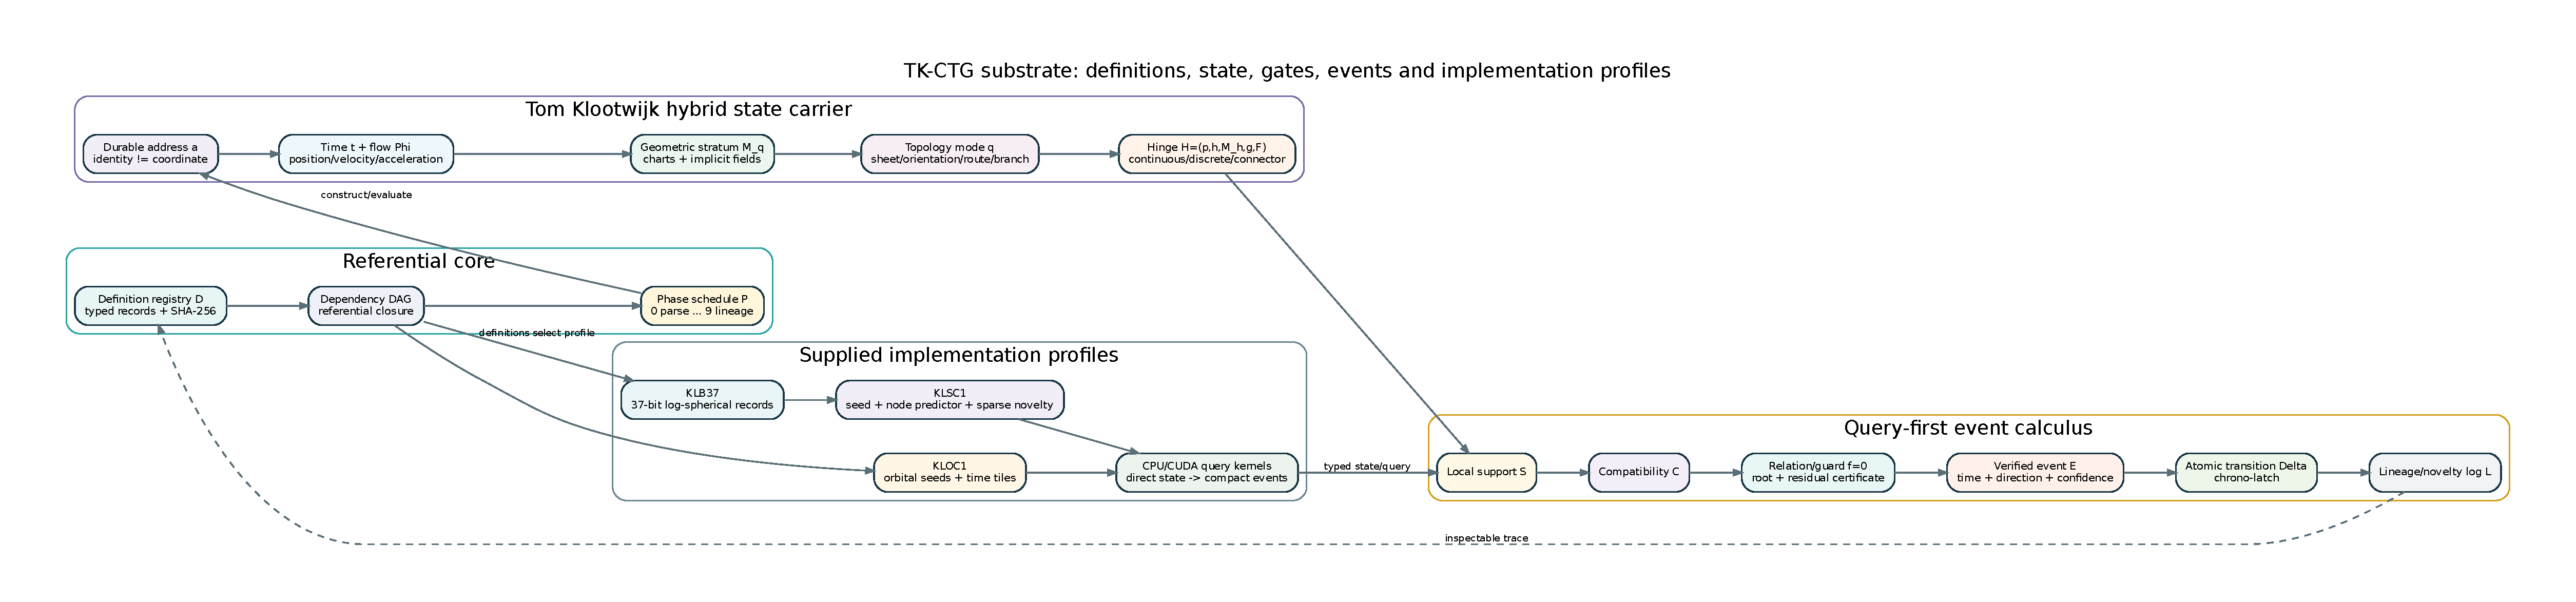
\includegraphics[width=\textwidth]{figures/ctg_architecture.pdf}
\caption{The definition registry selects a state/profile; the query path applies support, compatibility and a certified relation before a chronotopological transition and lineage append. This is an original diagram for this package, based on the source diagrams in UGTS-KC 3.6.}
\label{fig:architecture}
\end{figure}

\subsection{Addressed hybrid state}

\begin{formaldef}{Addressed state}{hybrid-state}
A runtime state is
\[
z=(a,t,q,\xi,\eta,\ell),
\]
where \(a\in\mathcal A\) is a durable address, \(t\in\Time\), \(q\in\mathcal Q\), \(\xi\in J^r(M_q)\) is a finite geometric jet (position and, when declared, velocity/acceleration or higher derivatives), \(\eta\) is auxiliary hinge/grammar/profile state, and \(\ell\) is ordered lineage.
\end{formaldef}

The state identity key is at minimum \((a,q,\ell)\). Coordinates are observations of state, not replacements for identity.

\begin{proposition}{Co-location does not imply state equality}{colocation}
Let \(z_1=(a_1,t,q_1,\xi_1,\eta_1,\ell_1)\) and \(z_2=(a_2,t,q_2,\xi_2,\eta_2,\ell_2)\). Even when their position coordinates are equal, \(x(\xi_1)=x(\xi_2)\), the states are equal only if the declared identity, mode, auxiliary and lineage equivalence rules also hold. In particular, different sheets or routes remain distinct unless a gluing/transition map identifies them.
\end{proposition}

\textit{Reason.} The product/disjoint-union construction carries the mode label independently of the geometric coordinates. Quotient equality is introduced only by an explicit relation in \(\Gamma\) or \(\Delta\). This formalizes the source rule that projected self-intersection or co-location is not automatically a physical collision or coupling.

\subsection{Minimum referential API}

A conforming implementation should expose the following logical operations, whether through Python, C++, a data service or an offline verifier:

\begin{center}
\begin{tabularx}{0.96\textwidth}{@{}L{52mm}Y@{}}
\toprule
\textbf{Operation} & \textbf{Semantics} \\
\midrule
\code{definition\_at(id)} & Return exact typed record and content hash \\
\code{definition\_order()} & Return deterministic phase-compatible dependency order \\
\code{verify\_definition(id)} & Recompute canonical SHA-256 \\
\code{instances\_of(id)} & Enumerate literal uses of a definition \\
\code{explain\_reference(id)} & Return dependencies, phase, capabilities, invariants and provenance \\
\code{trace(pipeline,instance)} & Return ordered definition IDs, typed intermediate outputs, gates, event and lineage \\
\code{state\_at(address,time)} & Reconstruct or retrieve addressed state under a declared profile \\
\code{next\_event(query)} & Return earliest certified event or a typed rejection reason \\
\bottomrule
\end{tabularx}
\end{center}

\section{The Tom Klootwijk Manifold}
\label{sec:manifold}

\subsection{Profile and carrier}

A manifold profile is
\[
\Pi=(\mathcal Q,\{M_q\},\{U_q\},\Gamma,\Delta,\Time,\mathcal R),
\]
where \(U_q\) contains finite/continuous auxiliary hinge state and \(\mathcal R\) contains regularity declarations.

\begin{formaldef}{Tom Klootwijk Manifold}{tkm}
The \textbf{Tom Klootwijk Manifold} for profile \(\Pi\) is the quotient/geometric realization
\[
\TKM(\Pi)=
\left(
\bigsqcup_{q\in\mathcal Q}
\Time\times M_q\times U_q\times\{q\}
\right)\Big/\sim_{\Gamma,\Delta}.
\]
The relation \(\sim_{\Gamma,\Delta}\) is generated only by:
\begin{enumerate}
  \item declared boundary-port gluing maps \(\gamma\in\Gamma\), including coordinate, orientation, sheet, route and lineage transport; and
  \item guarded transition maps \(\delta\in\Delta\) applied on certified event strata.
\end{enumerate}
Durable addresses and full lineage label points/states over this carrier but are not silently collapsed into geometric coordinates.
\end{formaldef}

\begin{figure}[H]
\centering
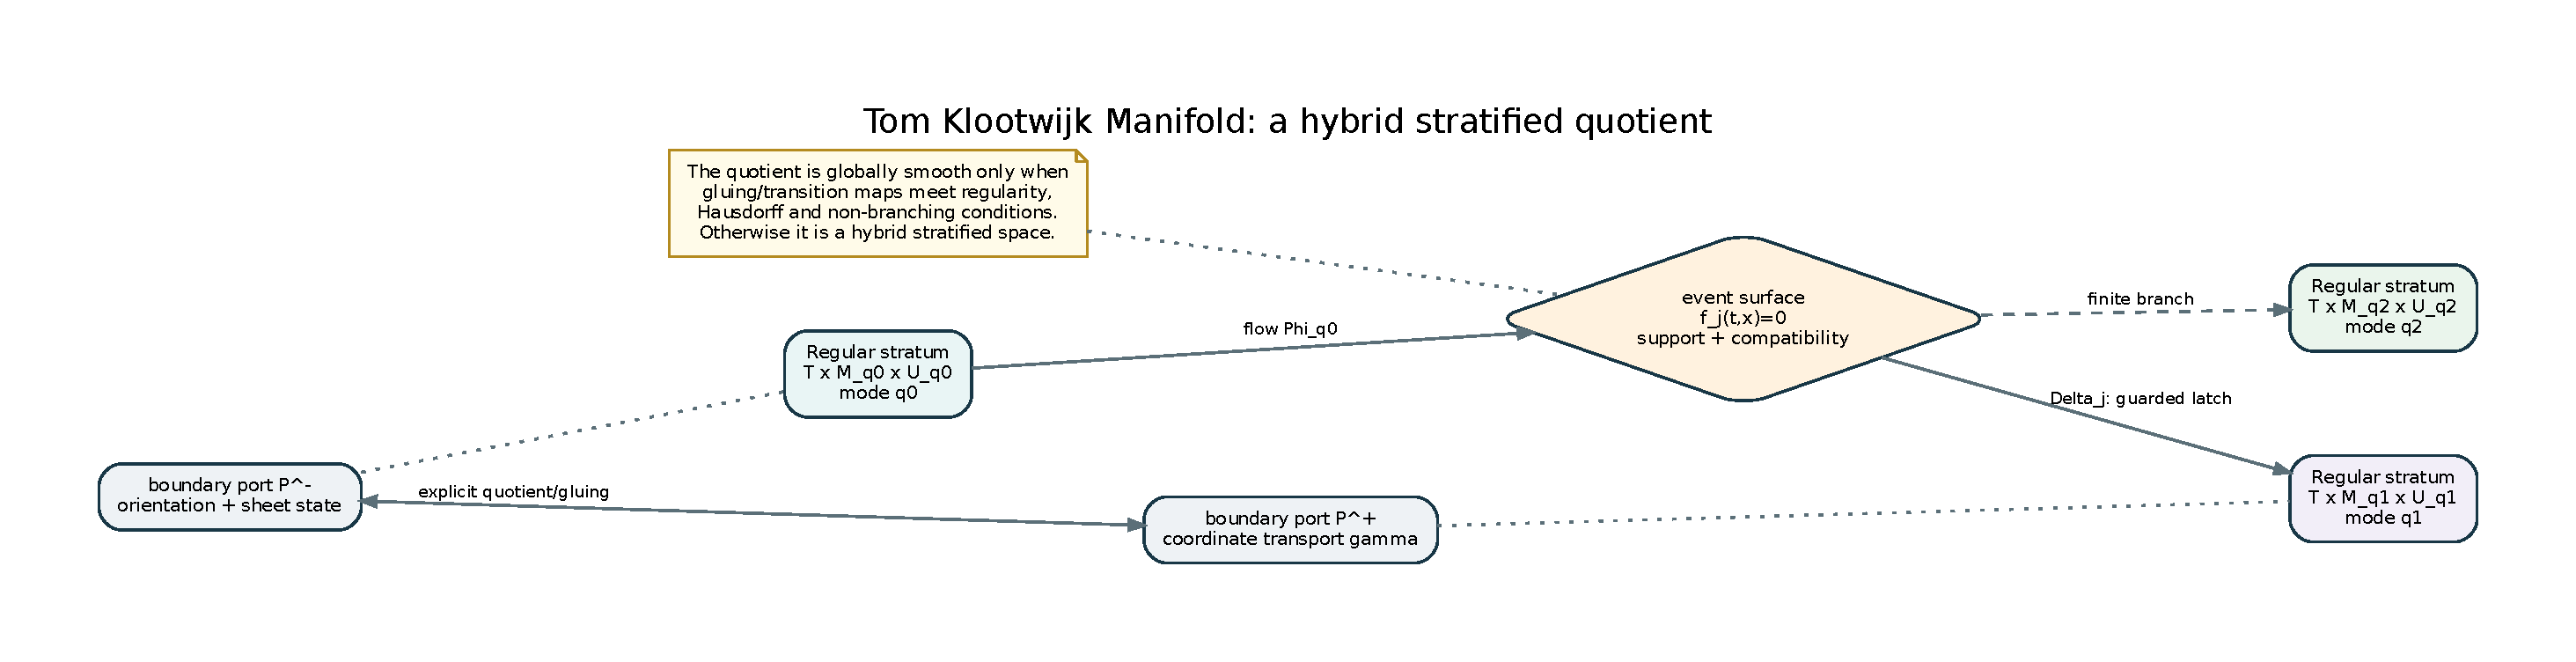
\includegraphics[width=\textwidth]{figures/tkm_manifold.pdf}
\caption{Regular time-extended strata are connected by explicit quotient ports and guarded event transitions. A finite branch makes the general object a hybrid stratified space rather than an automatically smooth manifold.}
\label{fig:tkm}
\end{figure}

\subsection{Why the formal class is hybrid and stratified}

For fixed \(q\), the regular carrier \(\Time\times M_q\times U_q\) may be a smooth manifold (or manifold with boundary) when \(U_q\) is smooth. Event sets
\[
\Sigma_{j,q}=\{(t,x,u): f_{j,q}(t,x,u)=0\}
\]
form lower-dimensional strata when \(0\) is a regular value. Gluing maps may reverse orientation or change sheet. Transition maps may branch, merge, reset state or append lineage. Such operations need not preserve the hypotheses required for a single global smooth manifold.

\begin{proposition}{Regular-manifold condition}{regularity}
Suppose: (i) every \(M_q\) and \(U_q\) is smooth; (ii) every active gluing map is a diffeomorphism between boundary components; (iii) the generated equivalence relation is proper and Hausdorff; (iv) no event produces branching or many-to-one merging; and (v) transition maps are smooth and compatible with local charts. Then the corresponding non-singular quotient component of \(\TKM(\Pi)\) is a smooth manifold (possibly with boundary/corners). If any condition fails, the formal object remains a valid hybrid stratified topological state space, but global smooth-manifold language must be qualified.
\end{proposition}

This qualification is not a weakness. It is exactly what allows the same substrate to represent ordinary smooth motion, quotient surfaces, discrete route sheets, event routers, frame/node chains and finite branches without pretending that they are one undifferentiated smooth geometry.

\subsection{Individual naming, not family folding}

The requested name refers to the precise construction in Formal Definition~\ref{def:tkm}. It does not mean every object associated with the surname Klootwijk, nor does it create a family-wide attribution. The formal identifier in the shipped JSON is \code{manifold:tom-klootwijk-v1}; the attribution block contains the exact requester-supplied name, identifier and date string, with status \code{requester-supplied-unverified}.

\section{Chronology, event surfaces and the chronotemporal latch}
\label{sec:chrono}

\subsection{Time and flow}

\begin{formaldef}{Mode-dependent flow or predictor}{flow}
For each mode \(q\), a flow/predictor is a typed map
\[
\Phi_q:(t,t_0,\xi_0,\theta_q)\longmapsto \xi(t)\in J^r(M_q),
\]
with declared time units, origin, parameter/profile version, iteration policy and error bound. A closed-form law, a fixed-step recurrence, a seed reconstruction or a bounded numerical solver may instantiate \(\Phi_q\).
\end{formaldef}

Time is therefore explicit. A 4-vector may include a homogeneous coordinate or an application-chosen time coordinate, but the symbol \((4,4,4,4)\) does not by itself define chronology. The substrate becomes chrono-topological because \(t\), \(\Phi\), event times, transition order and lineage are part of the typed state.

For constant acceleration, one permitted profile is
\[
x(t)=x_0+v_0\Delta t+\tfrac12a\Delta t^2,
\qquad v(t)=v_0+a\Delta t.
\]
The KLSC1 profile stores time, angle, angular velocity and angular acceleration in each node. The KLOC1 profile stores a common epoch, time tiles and a deterministic orbital predictor.

\subsection{Relation guard and earliest event}

\begin{formaldef}{Certified chrono-topological event}{cert-event}
Let \(f_j(z(t))\) be a scalar relation guard. The next event is
\[
t^*=\inf\left\{t>t_0:
\begin{array}{l}
 f_j(z(t))=0,\\
 S_\alpha(z(t),t)=1,\\
 C(z(t),j,t)=1,\\
 \operatorname{conf}(t)\ge\operatorname{conf}_{\min},\\
 \varepsilon_{\mathrm{num}}<m_{\mathrm{guard}}
\end{array}
\right\},
\]
provided a solver or sampled crossing certificate establishes existence, direction and residual within the declared interval. The event record contains the pre-state, post-state proposal, relation ID, residual, crossing direction, solver status, support/compatibility result, confidence, route and lineage references.
\end{formaldef}

For adjacent sampled values \(g_0,g_1\), the KLOC1-style certificate uses:
\[
(g_0>0\wedge g_1\le0)\ \vee\ (g_0\le0\wedge g_1>0),
\]
requires \(\min(|g_0|,|g_1|)\) to lie in a declared crossing band, requires support/compatibility gates, and estimates
\[
\lambda=\operatorname{clamp}\!\left(\frac{g_0}{g_0-g_1},0,1\right),
\qquad t^*=t_0+\lambda(t_1-t_0).
\]

\subsection{Chronotemporal latch}

\begin{formaldef}{Chronotemporal latch}{latch}
Let \(q(t)\) be the discrete topology/mode component. Between certified events,
\[
q(t)=q_k,\qquad t\in[t_k^*,t_{k+1}^*).
\]
At a verified event \(e_j\) at time \(t^*\), commit atomically
\[
z(t^{*+})=\Delta_j(z(t^{*-}),e_j),
\]
append the transition to lineage, and set the declared latch state. A one-shot scalar representation is \(\lambda_j(t)=\mathbf 1[t\ge t^*]\); multi-state latches use a finite state machine.
\end{formaldef}

This is the rigorous interpretation of the phrase \emph{higher-order definition compounded on this latches the substrate chronotemporally}. The latch is neither a teleportation theorem nor automatic anti-aliasing. It is a state-machine guarantee: discrete topology does not drift continuously; it changes at an explicitly certified time and records the change.

\begin{figure}[H]
\centering
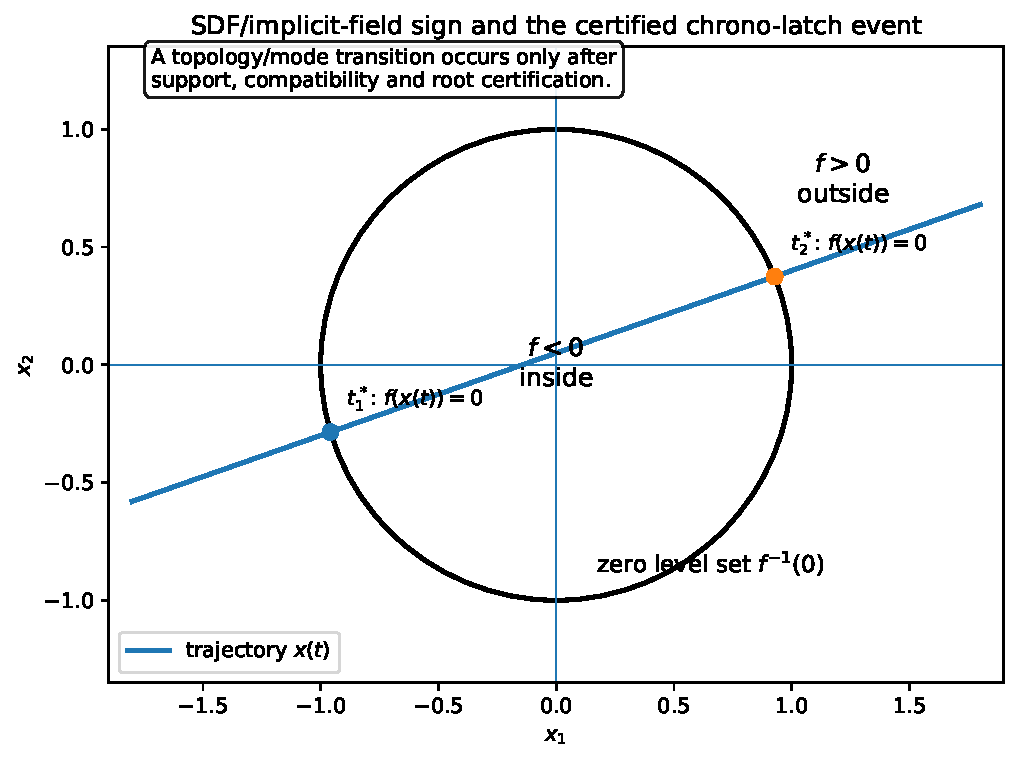
\includegraphics[width=0.92\textwidth]{figures/sdf_chrono_latch.pdf}
\caption{An implicit field supplies sign and a zero-level event surface. The transition is committed only after support, compatibility and root certification.}
\label{fig:sdf-latch}
\end{figure}

\begin{proposition}{Piecewise-constant mode and deterministic event trace}{piecewise}
Assume each flow \(\Phi_q\), predicate, solver tie-break rule and transition is deterministic; all definitions and parameters are fixed; and each event interval has a unique earliest admissible root. Then \(q(t)\) is piecewise constant and the ordered event/lineage trace is unique for a given initial state and query.
\end{proposition}

\textit{Proof sketch.} Induct on event count. The deterministic flow uniquely determines the pre-event trajectory. The support and compatibility predicates determine the admitted relation set. The unique earliest-root/tie-break rule determines \(t^*\) and event ID. The deterministic atomic transition determines the next state. Repeat.

\section{Geometric calculus and SDF boundary}
\label{sec:geometry}

\subsection{Parametric and implicit definitions}

A parametric definition is
\[
\gamma:U\to\Real^n,\qquad u\mapsto\gamma(u),
\]
with declared interval/domain, regularity and frame policy. An implicit definition is
\[
f:\Real^n\to\Real,
\quad f(x)<0\ \text{inside},\quad f(x)=0\ \text{boundary},\quad f(x)>0\ \text{outside}.
\]
The sign convention is structural: it supports membership tests, CSG sign composition and event guards.

For two sign fields,
\[
f_{A\cup B}=\min(f_A,f_B),\quad
f_{A\cap B}=\max(f_A,f_B),\quad
f_{A\setminus B}=\max(f_A,-f_B).
\]
These identities preserve sign semantics, not necessarily exact-distance semantics.

\subsection{Exact SDF is a capability}

\begin{formaldef}{Exact signed-distance capability}{exact-sdf}
For a declared closed set/boundary, an exact signed-distance function returns the signed Euclidean distance to the boundary under the profile’s metric. Exactness must be established by the primitive/transform definition. A generic implicit field, smoothed blend, fractal estimator or arbitrary morph may carry correct sign without carrying exact distance. Where differentiable, \(\|\nabla d\|=1\) is a characteristic property of exact Euclidean distance, but it is not a universal declaration generated by the letters SDF.
\end{formaldef}

A sphere centered at \(c\) with radius \(r>0\) is specifically
\[
f_{\mathrm{sphere}}(x)=\|x-c\|-r.
\]
Only with this or an equivalent declared field does \(f=0\) define that sphere. In general, \(f=0\) defines whatever zero-level set the function encodes.

\subsection{Rounded/fractal profile}

Let \(F\subset\Real^n\) be a declared closed fractal, point set or procedural set. An explicit offset profile is
\[
f_\epsilon(x)=d(x,F)-\epsilon,
\qquad F_\epsilon=\{x:d(x,F)\le\epsilon\}.
\]
This thickens the set and can produce a visually rounded envelope. It does not guarantee global smoothness: offset boundaries can be non-differentiable at medial-axis or self-contact loci. Additional convolution, a smooth-min field, a curvature flow or another regularizer must be named if smoother behavior is required.

\begin{boundarybox}
\textbf{Sierpinski/Mandelbulb language is profile metadata, not the core.} A Sierpinski parity mask, iterated-function system, distance estimator or 3D fractal can be added as a bounded geometric definition. None is implied merely by writing \((4,4,4,4)\), \code{SDF 0}, \code{(3)} or an LSB selector. The current KLB implementation uses log-spherical point records, a finite parity grammar and a discrete Klein routing map; it is not an exact Mandelbulb renderer.
\end{boundarybox}

\subsection{Optional seven-axis profile}

\begin{formaldef}{TK7 orthogonality profile}{tk7}
Set \(M_q=\Real^7\) with the standard inner product. For \(i=0,\ldots,6\), let
\[
L_i=\{c+\lambda e_i:\lambda\in\Real\},
\]
where \(e_i\) are the seven standard basis vectors. Then the seven axis lines are pairwise orthogonal.
\end{formaldef}

This is the precise, standard way to satisfy the \emph{seven mutually perpendicular directions} motif. It is optional. It does not follow from a four-dimensional vector or from a bit/fold notation, and the supplied KLB37/KLSC1 point path remains a three-coordinate implementation unless extended.

\section{Topology, quotient maps and hinges}
\label{sec:topology}

\subsection{Explicit gluing}

\begin{formaldef}{Port gluing}{gluing}
A topology/gluing record is
\[
G_i=(P_i^-,P_i^+,\gamma_i,\omega_i,\sigma_i,\rho_i,\ell_i),
\]
where \(P_i^-\) and \(P_i^+\) are named ports, \(\gamma_i\) transports coordinates, \(\omega_i\) transports orientation, \(\sigma_i\) updates sheet, \(\rho_i\) updates route/branch state, and \(\ell_i\) updates lineage. Only this record creates the corresponding quotient identification.
\end{formaldef}

A continuous geometric projection may show two branches crossing. That picture does not identify their addressed states. The topology component records whether they are the same point, different sheets, incompatible routes or merely a visual overlap.

\subsection{Generic hinge}

\begin{formaldef}{Hinge}{hinge}
A hinge is
\[
H=(p,h,M_h,g,F),
\]
where \(p\) is a pivot or connector locus, \(h\) is continuous or discrete hinge state, \(M_h\) is the selected map, \(g\) is the state-change guard, and \(F\) is a declared invariant/fixed set.
\end{formaldef}

A planar continuous hinge about pivot \(p\) uses
\[
x'(t)=p+R(\theta(t))(x-p),
\qquad
\dot{x}'(t)=\dot\theta(t)J R(\theta(t))(x-p).
\]
A parity hinge selects \(M_0\) or \(M_1\) only after a declared guard. A connector hinge may have zero numeric magnitude but nonzero graph/topological role. Composition order is literal and generally non-commutative:
\[
H_2\circ H_1\ne H_1\circ H_2.
\]

\subsection{Discrete Klein profile}

For integer grid dimensions \(W,H>0\), let
\[
m=\left\lfloor \frac{y}{H}\right\rfloor,
\qquad \bar y=y\bmod H,
\qquad \epsilon=m\bmod 2.
\]
Then
\[
\bar x=
\begin{cases}
x\bmod W,&\epsilon=0,\\
(W-1-x)\bmod W,&\epsilon=1.
\end{cases}
\]
The map returns \((\bar x,\bar y,\epsilon)\), where \(\epsilon\) is the reflection/orientation bit. Equivalently,
\[
K(x+W,y)=K(x,y),
\qquad K(x,y+H)=K(W-1-x,y).
\]
This is exactly the bounded logical map in the supplied implementation. It never permits out-of-range memory access and does not claim that physical VRAM has Klein-bottle topology.

\subsection{XOR tile swizzle}

Inside a \(16\times16\) logical tile, with row \(r\) and column \(c\), the implementation uses
\[
\sigma(r,c)=(r,c\oplus r).
\]
Since \((c\oplus r)\oplus r=c\), \(\sigma\) is self-inverse. It is an explicit permutation of addresses in the application buffer, not a claim about undocumented hardware tiling.

\section{Implementation profile A: KLB37 and KLSC1}
\label{sec:klsc1}

\begin{implementationbox}
\textbf{Purpose.} Reconstruct a time-varying point state on demand from one packed base, deterministic node state and sparse external novelty, then evaluate local events without requiring the complete dense sequence in VRAM.
\end{implementationbox}

\subsection{KLB37 record and chart}

A logical record is
\[
c=(q_\rho,q_\theta,q_\phi,s,p),
\]
with bit widths \(11,12,10,3,1\), totaling 37 bits. The parity bit is selected so the complete record has even parity. Records are concatenated continuously and may cross word boundaries.

For decode parameters center \(c_0\), scale \(R\), and \(k>0\), set
\[
\rho_n=\frac{q_\rho}{2^{11}-1},\qquad
\theta=\frac{2\pi q_\theta}{2^{12}},\qquad
\phi=\pi\left(\frac{q_\phi}{2^{10}-1}-\frac12\right),
\]
\[
r=R\frac{\exp(\rho_n\ln(1+k))-1}{k},
\]
and
\[
x=c_0+r(\cos\phi\cos\theta,\ \sin\phi,\ \cos\phi\sin\theta).
\]
The code stores a point approximation, a 3-bit symbol and parity. It does not store faces, normals, materials or a complete mesh.

\subsection{KLSC1 node and novelty state}

The canonical file layout is
\[
256+96F+16N+4W\quad\text{bytes},
\]
where \(F\) is node/frame count, \(N\) novelty-record count and \(W\) embedded KLB37 word count. Each 96-byte node stores parent/frame IDs, seed/flags, time, angle, angular velocity/acceleration, log-scale, translation, cone phase, branch amplitude, novelty range, checkpoint metadata and parent/self hashes. Each 16-byte novelty record stores stable point index, signed quantized \((dx,dy,dz)\), flags and event seed.

\subsection{Reconstruction map}

For point index \(i\) and target node \(n\), the implementation realizes a bounded map of the form
\[
\widehat p_{i,n}
=c_0+s_nR_y(\alpha_n)
\left[(p_i^0-c_0)+d_{i,n}^{\mathrm{grammar}}\right]
+\tau_n
+\sum_{m\in\operatorname{path}(n,cp(n))}\nu_{m,i}.
\]
Here:

\begin{enumerate}
  \item \(p_i^0\) is the decoded KLB37 base point;
  \item a fixed four-level parity grammar derives symbol and route;
  \item the discrete Klein map derives wrapped coordinate and orientation;
  \item a bounded cone/grammar deformation supplies \(d_{i,n}^{\mathrm{grammar}}\) for generated nodes;
  \item \(s_n=2^{\mathrm{log2\_scale}_n}\), \(R_y(\alpha_n)\) and \(\tau_n\) are absolute predictor fields;
  \item \(\nu_{m,i}\) is found by binary search in a sorted novelty range;
  \item the parent walk stops at a checkpoint and is capped at 64 nodes.
\end{enumerate}

The exact implementation’s cone field is an analytic infinite-cone sign field used as a deformation driver. It is not claimed to be an exact finite capped-cone distance.

\begin{proposition}{Bounded random-access reconstruction}{bounded-replay}
Let checkpoint stride be \(C\le64\), and let the largest novelty range searched contain \(N_{\max}\) records. The novelty portion of one point reconstruction requires at most \(C\) node visits and \(O(C\log N_{\max})\) comparisons. With fixed profile bounds this is constant with respect to total frame count, but it is not zero cost and its constant can dominate a dense resident query.
\end{proposition}

\subsection{Point event query}

The KLSC1 direct query reconstructs a point and evaluates:
\[
\begin{aligned}
S &= [r\le r_{\max}]\wedge[\widehat x\cdot a/r\ge\cos\alpha],\\
C &= [\text{route filter is any}]\vee[\text{route}=\text{filter}],\\
\mathrm{sdf} &= r-r_s,\\
g &= |\mathrm{sdf}|-\epsilon,\\
\mathrm{verified} &= S\wedge C\wedge[g\le0].
\end{aligned}
\]
A verified compact record contains point index, lineage/route and the SDF/guard values. This is a state-and-event profile, not a renderer.

\subsection{Integrity and precision contract}

KLSC1 uses a parent/self FNV-1a chain for deterministic integrity. Root parent hash commits to the embedded base payload; each next node commits to the previous self hash and its novelty bytes. FNV-1a is not a signature.

The precision contract is application-facing:
\[
\varepsilon_{\mathrm{base}}+\varepsilon_{\mathrm{predictor}}+
\varepsilon_{\mathrm{novelty}}+\varepsilon_{\mathrm{solver}}
<m_{\mathrm{event}}.
\]
Position RMS alone is insufficient when event membership or order can change near a guard.

\section{Implementation profile B: KLOC1 orbital seed timeline}
\label{sec:kloc1}

\begin{implementationbox}
\textbf{Purpose.} Store compact OMM-derived orbital seeds and a hash-linked time partition, reconstruct coarse satellite state on demand, apply station support/route compatibility, and emit bounded elevation-mask crossings.
\end{implementationbox}

\begin{figure}[H]
\centering
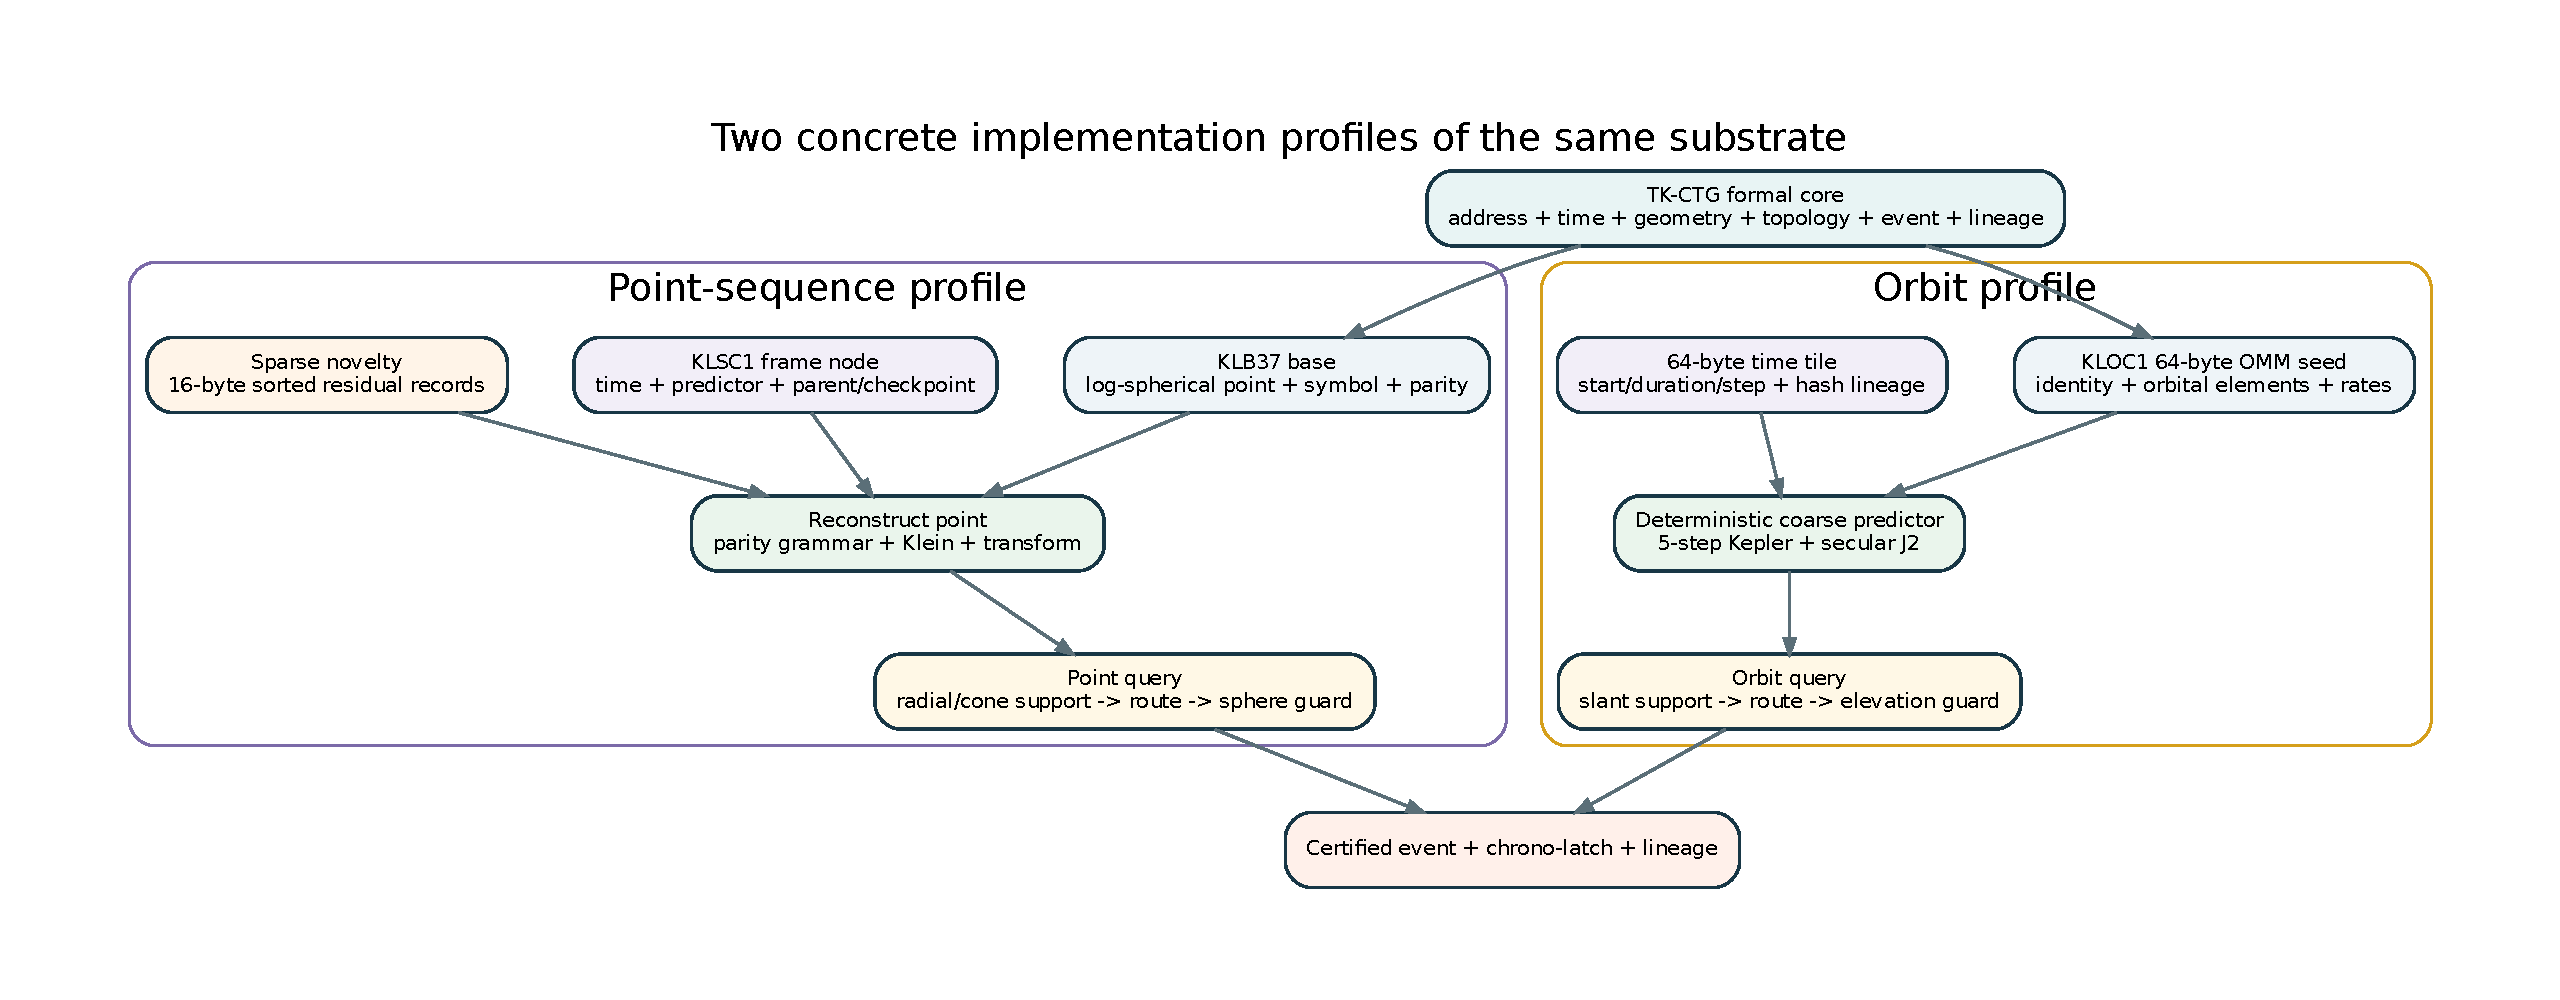
\includegraphics[width=\textwidth]{figures/implementation_bridge.pdf}
\caption{KLSC1 and KLOC1 are two different profiles of the same address--time--geometry--topology--event--lineage substrate.}
\label{fig:profiles}
\end{figure}

\subsection{KLOC1 records}

Version 1 has a 256-byte header, 64-byte seed records, 64-byte timeline nodes and a UTF-8 string table. A seed stores stable NORAD identity, PRN/route metadata, epoch offset, semi-major axis, eccentricity, inclination, RAAN, argument of perigee, mean anomaly, mean motion, secular rates, lineage seed and name offset. A timeline node stores parent/index, flags, chain seed, start/duration/step, parent/self/source hashes and sample range.

The six route sectors are deterministic RAAN bins used as a compatibility workload. They are not official orbital-plane labels.

\subsection{Deterministic coarse flow}

For \(\Delta t=t-t_{\mathrm{epoch}}\), the implementation updates RAAN, argument of perigee and mean anomaly using stored secular rates. It solves
\[
E-e\sin E=M
\]
with five fixed Newton iterations, then computes
\[
x_o=a(\cos E-e),\qquad
y_o=a\sqrt{1-e^2}\sin E,
\]
and rotates the perifocal coordinates into ECI using RAAN, inclination and argument of perigee.

This fixed iteration count makes the benchmark’s host/device work bounded and repeatable. The model is explicitly \code{kepler\_j2\_secular\_coarse}; CelesTrak general-perturbations elements are intended for SGP4, so this predictor is not navigation-grade.

\subsection{Station support, compatibility and guard}

Let \(s(t)\) be satellite ECI position and \(g(t)\) station ECI position after Earth rotation. Define line of sight \(\ell=s-g\), slant range \(r=\|\ell\|\), station zenith \(z=g/\|g\|\), and
\[
\sin e=\frac{\ell\cdot z}{\|\ell\|}.
\]
Then
\[
S=[r\le r_{\max}],
\quad C=[\text{route filter admits seed sector}],
\quad f=\sin e_{\min}-\sin e.
\]
An acquisition event is a verified crossing from \(f>0\) to \(f\le0\); a loss event is the reverse.

\subsection{Accuracy boundary}

\begin{boundarybox}
KLOC1 is a legitimate compact state/event benchmark and coarse scheduling profile. It is not an authoritative ephemeris. It must not be used for navigation, collision avoidance, safety of flight, tight antenna pointing or any application whose error/event-order budget has not been validated against SGP4 or a stronger reference.
\end{boundarybox}

The supplied independent-laptop report records a narrow direct-seed versus materialize-plus-query crossover for some one-off workloads, while a dense timeline already resident in VRAM remains substantially faster for repeated queries. It also records a full-horizon CPU/GPU support-count discrepancy of one interval and the absence of SGP4 validation. Those findings reinforce the formal rule: storage ratio alone is not acceptance; equal-accuracy event behavior and resource cost decide promotion.

\section{Phase-ordered evaluator and deterministic trace}
\label{sec:evaluator}

\begin{figure}[H]
\centering
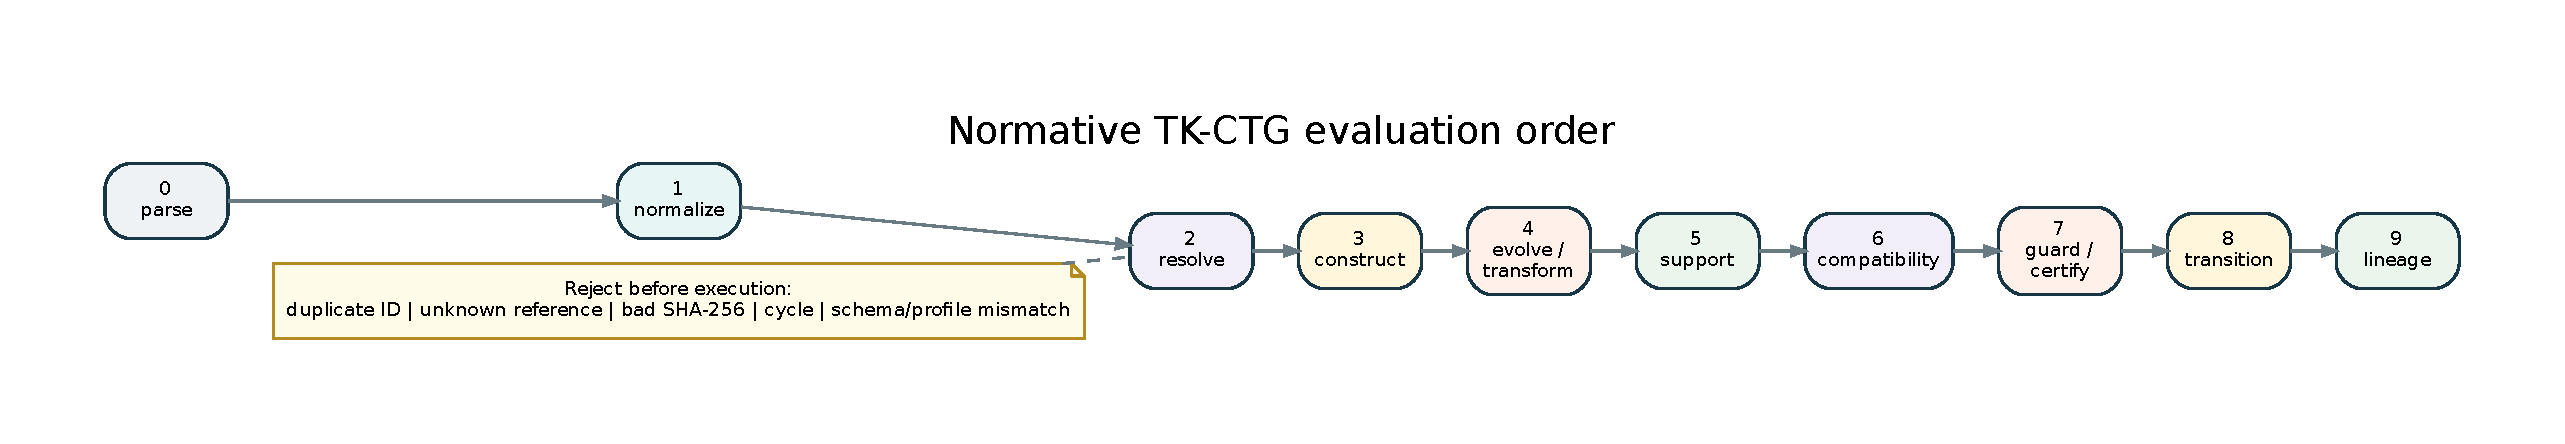
\includegraphics[width=\textwidth]{figures/phase_schedule.pdf}
\caption{Normative evaluation order. Definition dependencies are topologically sorted inside phase barriers.}
\label{fig:phase}
\end{figure}

\begin{longtable}{@{}C{12mm}L{32mm}L{113mm}@{}}
\toprule
\textbf{Phase} & \textbf{Name} & \textbf{Normative rule} \\
\midrule
\endfirsthead
\toprule
\textbf{Phase} & \textbf{Name} & \textbf{Normative rule} \\
\midrule
\endhead
0 & Parse & Parse literals, schemas, profiles and binary headers. \\
1 & Normalize & Normalize units, dimensions, profile versions and sign/frame conventions. \\
2 & Resolve & Resolve references, verify SHA-256 definitions, validate binary integrity and topologically sort dependencies. \\
3 & Construct & Construct geometric objects, charts, addresses, seeds, node/time partitions and query objects. \\
4 & Evolve/transform & Evaluate flow/predictor; apply ordered coordinate transforms, hinges and gluing maps. \\
5 & Support & Apply cheap local support predicates. \\
6 & Compatibility & Apply sheet, orientation, route, branch, profile and policy compatibility. \\
7 & Guard/certify & Solve or bracket roots; certify residual, direction, confidence and numerical margin. \\
8 & Transition & Commit topology/mode change atomically. A visual/field morph alone does not commit a topology change. \\
9 & Lineage & Append event, pre/post state, definition trace, parentage and novelty/log data. \\
\bottomrule
\end{longtable}

\begin{proposition}{Referential execution determinism}{determinism}
If the definition DAG is valid, hashes verify, all phase-local operations are deterministic, composition order is literal, and event tie-break rules are total, then an input document plus initial state and query yields a unique typed trace.
\end{proposition}

\textit{Proof sketch.} The definition order is unique under the declared deterministic sort. Induct over phases. Each phase consumes fixed prior typed outputs and emits fixed outputs; transition is delayed until all gates and certification are fixed; lineage appends the resulting trace without modifying earlier phases.

\section{Formal invariants}
\label{sec:invariants}

\begin{invariant}{Referential closure}{ref-closure}
Every definition and instance reference resolves to one stable ID; every definition content hash verifies; and the selected dependency graph is acyclic.
\end{invariant}

\begin{invariant}{Coordinate/identity separation}{identity}
Address, mode/sheet/route and lineage remain explicit even when coordinates coincide.
\end{invariant}

\begin{invariant}{Topology explicitness}{topology-explicit}
No projected overlap, bit pattern or storage address creates a topological identification unless a gluing or transition record declares it.
\end{invariant}

\begin{invariant}{Support before expensive relation solving}{gate-order}
Support is evaluated before compatibility, and both precede guard/root certification.
\end{invariant}

\begin{invariant}{Guarded topology change}{guarded-topology}
Continuous geometry may vary in phase 4, but mode/topology state changes only in phase 8 after a certified event.
\end{invariant}

\begin{invariant}{Precision margin}{precision}
The aggregate reconstruction and solver error must remain below the declared event margin; otherwise the event result is not accepted.
\end{invariant}

\begin{invariant}{Bounded replay}{replay}
A seed/log profile declares depth, checkpoint, symbol, expression and cycle budgets. KLSC1 version 1 caps checkpoint stride at 64.
\end{invariant}

\begin{invariant}{Narrow bit semantics}{bit}
A one-bit value selects a declared binary state, route, mask or validity condition. Continuous geometry, full identity and arbitrary numeric mutation remain separate.
\end{invariant}

\begin{invariant}{Attribution non-causality}{attribution}
Requester identity metadata may appear in provenance records but never changes the mathematical result unless an explicit, independently justified application parameter maps it into state.
\end{invariant}

\section{Validation and implementation status}
\label{sec:validation}

\subsection{Checks performed for this package}

The supplied KLB archive was extracted and its own SHA-256 manifest was checked: all 82 listed files matched. A fresh CPU-only CMake build was performed in the preparation environment, and both supplied C++ test suites passed. The new Python reference package validates the JSON Schema, verifies all 21 definition hashes, rejects cycles, checks KLB37 parity/roundtrip behavior, verifies XOR/Klein topology, certifies chrono-latches, checks the TK7 axes and enforces checkpoint bounds.

\begin{center}
\begin{tabularx}{0.94\textwidth}{@{}L{56mm}L{35mm}Y@{}}
\toprule
\textbf{Validation} & \textbf{Result} & \textbf{Scope} \\
\midrule
Supplied KLB manifest & 82/82 pass & SHA-256 file integrity for files listed by the source package \\
Supplied C++ CPU tests & 2/2 suites pass & KLB37/KLSC1 and KLOC1 host behavior in current environment \\
New TK-CTG reference tests & 19/19 pass & Schema, hashes, DAG, geometry, topology, events, latch and bounds \\
GPU execution in this preparation environment & Not run & No new CUDA/RTX performance claim is made here \\
PDF visual verification & Rendered and inspected & Layout/glyph/page checks recorded in validation report \\
\bottomrule
\end{tabularx}
\end{center}

\subsection{What the tests establish}

They establish internal consistency of the defined package and a concrete correspondence with the supplied CPU implementation. They do not establish a new physical theory, a universal linguistic/numerical law, legal authorship priority, cryptographic identity, zero-cost graphics, navigation-grade orbital accuracy or performance on hardware not run in this preparation environment.

\subsection{Reproduction commands}

\begin{lstlisting}[language=bash]
PYTHONPATH=src python -m unittest discover -s tests -v
PYTHONPATH=src python examples/demo.py

# Supplied C++ implementation, CPU-only verification:
cmake -S . -B build-cpu -DCMAKE_BUILD_TYPE=Release -DKLB_BUILD_CUDA=OFF
cmake --build build-cpu -j
ctest --test-dir build-cpu --output-on-failure
\end{lstlisting}

\section{Claims ledger}
\label{sec:claims}

The full machine-readable ledger is shipped as CSV and JSON. The table below is normative for the formal core.

\small
\begin{longtable}{@{}L{52mm}L{24mm}L{85mm}@{}}
\toprule
\textbf{Claim} & \textbf{Disposition} & \textbf{Formal treatment} \\
\midrule
\endfirsthead
\toprule
\textbf{Claim} & \textbf{Disposition} & \textbf{Formal treatment} \\
\midrule
\endhead
\bottomrule
\endlastfoot
The name/identifier/date define geometric constants. & REJECT & They are requester-supplied provenance metadata only. \\
Four homogeneous coordinates provide seven mutually perpendicular axes. & REJECT & At most four mutually orthogonal nonzero directions exist in Euclidean R\textasciicircum{}4. \\
A declared R\textasciicircum{}7 profile can contain seven orthogonal axis lines. & BOUNDED & The seven standard basis axes are pairwise orthogonal; this is independent of SDF or LSB notation. \\
SDF=0 defines a sphere. & CORRECTED & It defines the zero level set of the chosen field; a sphere requires f(x)=||x-c||-r. \\
Every implicit field is an exact signed-distance function. & REJECT & Exact-distance status is an explicit capability and can fail after generic morphs/blends. \\
SDF=0 automatically smooths a fractal or removes jaggedness. & REJECT & Rounding requires an explicit offset/filter/blend and may still have singularities. \\
LSB or zero-based indexing reduces the Hamming distance between 943 and 937. & REJECT & Indexing changes labels/access rules, not the numeric bit difference. \\
A parity bit may select one of two declared maps/routes. & SUPPORTED & This is the narrow parity-hinge semantics used by the implementation. \\
A parity bit by itself performs arbitrary multi-bit mutation. & REJECT & Route selection and numeric mutation are distinct operations. \\
Chronology is obtained merely by treating w as time. & CORRECTED & The substrate declares a time domain, flow/predictor, event solver and transition record. \\
The chronotemporal latch makes topology state piecewise constant between events. & ENGINEERING & This is the formal interpretation adopted here. \\
Compact notation gives zero-byte VRAM and constant-time infinite rendering. & REJECT & Code and state still occupy memory and reconstruction has measurable ALU, cache and control cost. \\
KLSC1/KLOC1 can avoid materializing a dense timeline for selected queries. & BOUNDED & Useful only when the model is reconstructible and reconstruction cost/error meet the application budget. \\
Topology is explicit gluing/routing rather than physical self-intersection or energy creation. & SUPPORTED & This is the core semantics used in UGTS and KLB. \\
The Tom Klootwijk Manifold is globally smooth in every profile. & CORRECTED & It is generally a hybrid stratified quotient; only regular strata are smooth manifolds under regularity assumptions. \\
FNV chain hashes prove authorship or identity. & REJECT & They are deterministic integrity checks, not signatures. \\

\end{longtable}
\normalsize

\section{Acceptance and kill criteria}
\label{sec:acceptance}

A target profile should be rejected, simplified or replaced when any of the following occurs:

\begin{enumerate}
  \item definitions cannot be normalized to typed domains/codomains, stable IDs and verifiable content addresses;
  \item unresolved references, duplicate IDs, ambiguous profiles or dependency cycles remain;
  \item operation order changes results but is not recorded;
  \item gluing/transition maps fail to declare orientation, sheet, route or lineage transport;
  \item support and compatibility do not prune enough work to justify the event architecture;
  \item numerical/reconstruction error approaches or exceeds the guard margin or changes event order;
  \item branch/event/novelty density makes compact state more expensive than the dense alternative;
  \item a one-bit selector is misrepresented as full state or arbitrary data mutation;
  \item optional fractal/7D/artistic profiles are presented as properties of the current 3D implementation without an extension;
  \item an application requires authoritative physics/ephemerides but the selected predictor is only coarse;
  \item a conventional representation is simpler, faster or more accurate at equal access/error requirements;
  \item attribution metadata is used as causal geometry or as a substitute for evidence.
\end{enumerate}

\begin{decisionbox}
\textbf{Promotion rule.} Use a compact TK-CTG profile when its definitions are verifiable, its state is reconstructible, its topology/event semantics are explicit, its error remains below the event margin, and its end-to-end resource cost is better for the intended query pattern. Otherwise use the simpler or denser model.
\end{decisionbox}

\section{Conclusion}
\label{sec:conclusion}

The formal thread across the supplied documents is not a hidden universal code. It is a disciplined method for carrying definitions, compact state, geometry, topology, time, event conditions and lineage in one inspectable substrate.

The \textbf{Tom Klootwijk Manifold} is the mode-indexed, time-extended quotient carrier of that substrate. Its regular pieces are geometric manifolds; its seams are explicit gluing maps; its event sets are relation level sets; and its discrete topology state is chronotemporally latched by certified transitions. The name is individual as requested. The rigorous category is hybrid and stratified whenever branch, merge, sheet or reset behavior prevents a single smooth global manifold.

The supplied KLB implementation fits the definition in two concrete ways. KLB37/KLSC1 reconstructs point-sequence state from packed log-spherical records, finite parity grammar, discrete Klein routing, node predictors and bounded sparse novelty. KLOC1 reconstructs coarse orbital state from fixed seeds and hash-linked time tiles, then applies support, route compatibility and an elevation guard. Both produce event records and lineage; neither turns topology into physics or compact notation into free computation.

\begin{decisionbox}
\textbf{Final formal definition.}
\[
\boxed{
\TKM(\Pi)=
\left(\bigsqcup_{q\in\mathcal Q}\Time\times M_q\times U_q\times\{q\}\right)/\sim_{\Gamma,\Delta}
}
\]
\[
\boxed{
\TKSub(\Pi)=
(\mathcal D,\mathcal A,\TKM(\Pi),\Phi,\mathcal F,\mathcal S,\mathcal C,
\mathcal H,\mathcal E,\Delta,\mathcal I,\mathcal L,\mathcal P,\mathcal B)
}
\]
with requester attribution \emph{Tom Klootwijk; NL200678942; 10-07-1990}, explicitly marked as requester-supplied provenance and not a mathematical invariant.
\end{decisionbox}

\appendix
\clearpage
\section{Complete operator catalog}
\label{app:operators}

\begingroup
\setlength{\tabcolsep}{4pt}
\scriptsize
\begin{longtable}{@{}L{10mm}L{22mm}L{30mm}L{75mm}L{21mm}@{}}
\toprule
\textbf{ID} & \textbf{Domain} & \textbf{Mechanism} & \textbf{Formal rule} & \textbf{Disposition} \\
\midrule
\endfirsthead
\toprule
\textbf{ID} & \textbf{Domain} & \textbf{Mechanism} & \textbf{Formal rule} & \textbf{Disposition} \\
\midrule
\endhead
\bottomrule
\endlastfoot
TK-01 & Referential core & Literal definition node & Store every geometry, topology, profile, event and schedule as a typed content-addressed record. & SOURCE-DERIVED \\
TK-02 & Referential core & Dependency closure & Reject unknown IDs, duplicate IDs, invalid hashes and cycles. & SOURCE-DERIVED \\
TK-03 & Identity & Coordinate/address separation & Retain durable address, mode and lineage separately from geometric coordinates. & SOURCE-DERIVED \\
TK-04 & Geometry & Parametric chart & Declare parameter domain, frame, regularity and codomain. & SOURCE-DERIVED \\
TK-05 & Geometry & Implicit sign field & Use negative/zero/positive for inside/boundary/outside. & SOURCE-DERIVED \\
TK-06 & Geometry & Exact-SDF capability & Claim exact distance only for definitions that establish it. & CORRECTED \\
TK-07 & Geometry & Fractal offset regularization & Round/thicken a declared set by d(x,F)-epsilon; do not infer smoothness automatically. & CORRECTED \\
TK-08 & Topology & Explicit quotient/gluing & Name ports, coordinate transport, orientation, sheet and lineage updates. & SOURCE-DERIVED \\
TK-09 & Topology & Sheet-aware co-location & Equal coordinates do not imply equality or coupling. & SOURCE-DERIVED \\
TK-10 & Topology & Discrete Klein route & Periodic x wrap plus y-seam x reflection and orientation bit. & SOURCE-DERIVED \\
TK-11 & Hinge & Generic hinge tuple & Use H=(pivot/state/map/guard/invariants) for continuous, discrete and connector hinges. & SOURCE-DERIVED \\
TK-12 & Chronology & Explicit time domain & Represent time as a declared coordinate/domain, not an implicit bit or homogeneous coordinate. & CORRECTED \\
TK-13 & Chronology & Deterministic flow & Use a versioned closed form or bounded predictor for state evolution. & ENGINEERING \\
TK-14 & Events & Local support gate & Prune candidates before compatibility and root solving. & SOURCE-DERIVED \\
TK-15 & Events & Compatibility gate & Admit only declared sheets/routes/branches/profiles. & SOURCE-DERIVED \\
TK-16 & Events & Certified relation crossing & Require root/sign evidence, guard band, direction, confidence and numerical margin. & SOURCE-DERIVED \\
TK-17 & Transitions & Chronotemporal latch & Keep mode state piecewise constant and change it atomically only at a verified event. & ENGINEERING \\
TK-18 & Lineage & Ordered event log & Append pre/post state, time, relation, residual, route, parents and definition trace. & SOURCE-DERIVED \\
TK-19 & Implementation & KLB37 record & Use 11/12/10/3/1 continuous log-spherical/symbol/parity bits. & SOURCE-DERIVED \\
TK-20 & Implementation & XOR tile swizzle & Use a self-inverse 16x16 logical address permutation. & SOURCE-DERIVED \\
TK-21 & Implementation & KLSC1 seed chain & Reconstruct from KLB37 base, fixed grammar, node predictor and bounded sparse novelty. & SOURCE-DERIVED \\
TK-22 & Implementation & KLOC1 timeline & Reconstruct coarse orbital state from 64-byte seeds and hash-linked time tiles. & SOURCE-DERIVED \\
TK-23 & Evaluation & Ten-phase evaluator & Parse, normalize, resolve, construct, evolve, support, compatibility, guard, transition, lineage. & ENGINEERING \\
TK-24 & Geometry profile & Seven-axis profile & R\textasciicircum{}7 supplies seven mutually orthogonal standard axes; this is optional and not the current R\textasciicircum{}3 KLB default. & BOUNDED \\
TK-25 & Complexity & Bounded replay & KLSC1 parent walk is bounded by checkpoint stride <=64; bounded is not zero-cost. & SOURCE-DERIVED \\
TK-26 & Integrity & Dual hash boundary & Use SHA-256 for definition content addressing and FNV-1a only for supplied binary-chain integrity. & ENGINEERING \\
TK-27 & Acceptance & Error-before-claim & Promote a profile only when reconstruction and solver error stay below the event margin at the required cost. & SOURCE-DERIVED \\

\end{longtable}
\endgroup

\section{JSON formal-instance excerpt}
\label{app:json}

The complete file \code{spec/tk\_ctg\_substrate\_definition.json} contains 21 content-addressed definitions, three instances, the ten-phase schedule and profile metadata. The following excerpt shows the document header and attribution boundary.

\lstinputlisting[language=json,firstline=1,lastline=35]{../spec/tk_ctg_substrate_definition.json}

\section{Package layout}
\label{app:layout}

\begin{lstlisting}
Tom_Klootwijk_CTG_Substrate_v1.0.0/
  README.md
  NOTICE.md
  VERSION
  pyproject.toml
  report/
    Tom_Klootwijk_CTG_Substrate_v1.0.0.pdf
    Tom_Klootwijk_CTG_Substrate_v1.0.0.tex
    figures/*.pdf, *.png, *.dot
  spec/
    tk_ctg_substrate.schema.json
    tk_ctg_substrate_definition.json
    operator_catalog.{csv,json}
    claims_ledger.{csv,json}
  src/tkctg/*.py
  tests/test_tkctg.py
  examples/demo.py
  examples/demo_output.json
  bridge/KLB_IMPLEMENTATION_MAPPING.md
  sources/source_register.json
  sources/SOURCE_MAPPING.md
  validation/*
  checksums/SHA256SUMS.txt
\end{lstlisting}

\section{Source hashes}
\label{app:hashes}

\begin{tabularx}{\textwidth}{@{}L{14mm}Y@{}}
\toprule
SRC-A & \texttt{e21433cd8378368dafe4ae278d3c9c364725e45ae7fd75b743328bd2d6003a46} \\
SRC-B & \texttt{5004ef709ddd2de3350069642fdd7c78f4cdf6aeea15a2e703b952766f6b97d2} \\
SRC-C & \texttt{b3ab8e1d9f47171efa4f8370c94f3b4a48b58eb5bf30970312c7573d249b6aa3} \\
SRC-D & \texttt{c3e00e94ff1c3c13ac9ae76ea84a95117551e022375cefda8c706a7bb14d1ad4} \\
\bottomrule
\end{tabularx}

\vfill
\begin{center}
\sffamily\small End of formal specification -- TK-CTG 1.0.0
\end{center}

\end{document}
